% chapter 5
\chapter{Results and Discussions}
In this chapter we will discuss the results from the analysis of benchmark datasets and the problem dataset, followed
by the discussions on the results. Finally, we give recommendation to the company based on the requirements stipulated
in chapter 3.

\section{Results}
Table 5.1 shows the result of the analysis of various benchmark datasets using Gurobi, or-tools and optaplanner. There is
a time limit imposed on each analysis. For gurobi and optaplanner, the model runs for approximately\footnote{need to account for the reaction
time of human} the full duration of time limit and whatever solution is retrieved at the end of it is recorded. For optaplanner, the tabulated
time is taken the moment its tabulated solution does not change. All solution stated is in terms of the total euclidian distance
of all routes combined.
\begin{table}[!ht]
\caption{results}
\label{table:results}
\begin{center}
\begin{tabular}{|l|l|l|l|l|l|l|}
\hline
\multirow{2}{*}{Model /\ Solver}                                                         & \multicolumn{2}{l|}{Gurobi}                              & \multicolumn{2}{l|}{or-tools}                      & \multicolumn{2}{l|}{Optaplanner}                       \\ \cline{2-7}
                                                                                         & Time                           & Solution                & Time                     & Solution                & Time                     & Solution                \\ \hline
\multirow{2}{*}{\begin{tabular}[c]{@{}l@{}}A-n32-k5\\ Best Solution: 784\end{tabular}}  & \multirow{2}{*}{leq 1s}        & \multirow{2}{*}{763.9}  & \multirow{2}{*}{< 1s} & \multirow{2}{*}{870.9}  & \multirow{2}{*}{11s}  & \multirow{2}{*}{787.1}  \\
                                                                                         &                                &                         &                          &                         &                              &                         \\ \hline
\multirow{2}{*}{\begin{tabular}[c]{@{}l@{}}A-n44-k6\\ Best Solution: 937\end{tabular}}   & \multirow{2}{*}{5 mins} & \multirow{2}{*}{849}    & \multirow{2}{*}{< 1s} & \multirow{2}{*}{1013.8} & \multirow{2}{*}{37s}  & \multirow{2}{*}{938.8}  \\
                                                                                         &                                &                         &                          &                         &                              &                         \\ \hline
\multirow{2}{*}{\begin{tabular}[c]{@{}l@{}}A-n53-k7\\ Best Solution: 1010\end{tabular}}  & \multirow{2}{*}{5 mins} & \multirow{2}{*}{925.9}  & \multirow{2}{*}{< 1s} & \multirow{2}{*}{1119.2} & \multirow{2}{*}{1:06} & \multirow{2}{*}{1057.3} \\
                                                                                         &                                &                         &                          &                         &                              &                         \\ \hline
\multirow{2}{*}{\begin{tabular}[c]{@{}l@{}}A-n65-k9\\ Best Solution: 1174\end{tabular}}  & \multirow{2}{*}{5 mins} & \multirow{2}{*}{1027}   & \multirow{2}{*}{< 1s} & \multirow{2}{*}{1284}   & \multirow{2}{*}{1:24} & \multirow{2}{*}{1187}   \\
                                                                                         &                                &                         &                          &                         &                              &                         \\ \hline
\multirow{2}{*}{\begin{tabular}[c]{@{}l@{}}A-n80-k10\\ Best Solution: 1763\end{tabular}} & \multirow{2}{*}{5 mins} & \multirow{2}{*}{1484.1} & \multirow{2}{*}{< 1s} & \multirow{2}{*}{1948.2} & \multirow{2}{*}{2:00} & \multirow{2}{*}{1797.6} \\
                                                                                         &                                &                         &                          &                         &                              &                         \\ \hline
\multirow{2}{*}{\begin{tabular}[c]{@{}l@{}}T-VRP-9\\ Best Solution: N.A\end{tabular}}    & \multirow{2}{*}{5 mins} & \multirow{2}{*}{34.6}   & \multirow{2}{*}{< 1s} & \multirow{2}{*}{34.7}   & \multirow{2}{*}{leq 1s}      & \multirow{2}{*}{31.5}   \\
                                                                                         &                                &                         &                          &                         &                              &                         \\ \hline
\multirow{2}{*}{\begin{tabular}[c]{@{}l@{}}P-VRP-60\\ Best Solution: N.A\end{tabular}}   & \multirow{2}{*}{5 mins} & \multirow{2}{*}{3.1}    & \multirow{2}{*}{< 1s} & \multirow{2}{*}{10.5}   & \multirow{2}{*}{1:04} & \multirow{2}{*}{2.9}    \\
                                                                                         &                                &                         &                          &                         &                              &                         \\ \hline
\end{tabular}
\end{center}
\end{table}

Based on the results above other considerations, we have decided to use oplaplanner to analyse the VRP problem.
We have analysed the CVRP and CVRPTW models based on the formulation in chapter 3 and tabulated the results in
table 5.2 below:
\begin{table}[!ht]
\centering
\begin{tabular}{|l|l|l|l|}
\hline
Model  & Time Window & Solution & Actual Distance \\ \hline
CVRP   & No          & 10.27   & 798.57\\ \hline
CVRPTW & Yes         & 10.49   & 828.95\\ \hline
\end{tabular}
\caption{Results of analysis of VRP problem}
\label{my-label}
\end{table}
Both models have the following parameters:
\begin{itemize}
\item P-VRP-227 dataset
\item Time limit of 5 mins
\item has 8 vehicles, each of which is capable of delivering 29 items.
\item 226 customers
\end{itemize}

For CVRPTW model, the earliest and latest time for delivery for all customers is set to 09:00 and 17:00 respectively. The
service time is set to 15 minutes.

These are the routes of the two models are tabulated in figure 5.3 and 5.4. The numbers represent the node number and
they are arranged in order of which customers get visited first.
\begin{table}[!ht]
\centering
\caption{Routes}
\label{my-label}
\begin{tabular}{|l|l|}
\hline
\multicolumn{2}{|l|}{CVRP Model}                                                                      \\ \hline
Vehicle No         & Order of visit                                                                         \\ \hline
\multirow{2}{*}{1} & \multirow{2}{*}{\begin{tabular}[c]{@{}l@{}}48, 57, 75, 70, 102, 87, 79, 96, 97, 91, 144, 126, 146, 145,\\ 163, 188, 182, 187, 171, 189, 143, 62, 156, 167, 134, 76, 45, 29\end{tabular}} \\
                   &                                                                                  \\ \hline
\multirow{2}{*}{2} & \multirow{2}{*}{\begin{tabular}[c]{@{}l@{}}24, 54, 68, 67, 85, 80, 110, 152, 180, 191, 193, 196, 181, 147,\\ 175, 113, 108, 83, 78, 130, 136, 154, 105, 73, 53, 23, 44, 41, 22\end{tabular}}  \\
                   &                                                                                  \\ \hline
\multirow{2}{*}{3} & \multirow{2}{*}{\begin{tabular}[c]{@{}l@{}}25, 40, 127, 107, 141, 199, 202, 209, 192, 213, 217, 222, 201,\\ 210, 208, 204, 206, 214, 207, 195, 205, 112, 92, 88, 104, 93\end{tabular}} \\
                   &                                                                                  \\ \hline
\multirow{2}{*}{4} & \multirow{2}{*}{\begin{tabular}[c]{@{}l@{}}32, 47, 59, 21, 26, 43, 31, 114, 98, 178, 172, 176, 161, 165,\\ 185, 216, 225, 218, 226, 227, 224, 220, 223, 215, 184, 103, 74, 63, 37\end{tabular}}  \\
                   &                                                                                  \\ \hline
\multirow{2}{*}{5} & \multirow{2}{*}{\begin{tabular}[c]{@{}l@{}}36, 60, 56, 128, 153, 140, 133, 166, 139, 162, 194, 183, 168,\\ 173, 155, 135, 115, 95, 72, 77, 94, 61, 99, 124, 86, 109, 123\end{tabular}}  \\
                   &                                                                                  \\ \hline
\multirow{2}{*}{6} & \multirow{2}{*}{\begin{tabular}[c]{@{}l@{}}71, 33, 69, 46, 42, 82, 65, 131, 132, 164, 169, 150, 177, 190,\\ 125, 116, 66, 118, 119, 106, 101, 138, 84, 90, 120, 142, 121, 111, 52\end{tabular}}  \\
                   &                                                                                  \\ \hline
\multirow{2}{*}{7} & \multirow{2}{*}{\begin{tabular}[c]{@{}l@{}}17, 20, 30, 19, 15, 13, 14, 35, 34, 38, 39, 28, 64, 58, 49, 51,\\ 55, 16, 18, 12, 50, 9, 10, 11, 7, 8, 2, 4, 5\end{tabular}}  \\
                   &                                                                                  \\ \hline
\multirow{2}{*}{8} & \multirow{2}{*}{\begin{tabular}[c]{@{}l@{}}3, 6, 89, 151, 129, 157, 122, 137, 159, 158, 117, 174, 198, 186,\\ 212, 211, 221, 219, 200, 203, 197, 179, 170, 149, 160, 148, 100, 81, 27\end{tabular}}  \\
                   &                                                                                  \\ \hline
\end{tabular}
\end{table}

\begin{table}[!ht]
\centering
\caption{Routes}
\label{my-label}
\begin{tabular}{|l|l|}
\hline
\multicolumn{2}{|l|}{CVRPTW Model}                                                                      \\ \hline
Vehicle No         & Order of visit                                                                           \\ \hline
\multirow{2}{*}{1} & \multirow{2}{*}{\begin{tabular}[c]{@{}l@{}}3, 151, 157, 85, 129, 122, 137, 159, 117, 158, 174, 136, 108, 95,\\ 113, 198, 179, 197, 203, 212, 211, 221, 219, 200, 89, 8, 7, 2\end{tabular}} \\
                   &                                                                                  \\ \hline
\multirow{2}{*}{2} & \multirow{2}{*}{\begin{tabular}[c]{@{}l@{}}24, 40, 41, 27, 81, 148, 110, 78, 72, 83, 80, 77, 115, 149, 186,\\ 191, 181, 196, 193, 152, 133, 61, 140, 94, 124, 99, 54, 44\end{tabular}}  \\
                   &                                                                                  \\ \hline
\multirow{2}{*}{3} & \multirow{2}{*}{\begin{tabular}[c]{@{}l@{}}25, 60, 56, 86, 100, 135, 166, 139, 155, 194, 162, 183, 173, 168,\\ 170, 160, 180, 175, 147, 130, 154, 105, 73, 68, 67, 53, 23, 36, 22\end{tabular}} \\
                   &                                                                                  \\ \hline
\multirow{2}{*}{4} & \multirow{2}{*}{\begin{tabular}[c]{@{}l@{}}55, 37, 63, 31, 93, 123, 109, 127, 141, 128, 153, 107, 199, 202,\\ 209, 192, 201, 210, 222, 217, 213, 204, 208, 205, 185, 172, 91, 104, 48\end{tabular}}  \\
                   &                                                                                  \\ \hline
\multirow{2}{*}{5} & \multirow{2}{*}{\begin{tabular}[c]{@{}l@{}}75, 102, 103, 145, 176, 184, 215, 220, 223, 224, 227, 226, 225,\\ 216, 218, 195, 214, 207, 206, 178, 161, 165, 112, 98, 92, 88, 114, 43, 26\end{tabular}}  \\
                   &                                                                                  \\ \hline
\multirow{2}{*}{6} & \multirow{2}{*}{\begin{tabular}[c]{@{}l@{}}52, 111, 118, 119, 106, 101, 142, 121, 120, 90, 84, 190, 177,\\ 116, 125, 164, 169, 150, 134, 132, 131, 82, 65, 76, 46, 69, 70, 57\end{tabular}}  \\
                   &                                                                                  \\ \hline
\multirow{2}{*}{7} & \multirow{2}{*}{\begin{tabular}[c]{@{}l@{}}32, 47, 59, 21, 87, 97, 126, 163, 146, 144, 188, 182, 187, 96,\\ 79, 74, 143, 62, 156, 189, 171, 167, 45, 42, 29, 33, 71\end{tabular}}  \\
                   &                                                                                  \\ \hline
\multirow{2}{*}{8} & \multirow{2}{*}{\begin{tabular}[c]{@{}l@{}}19, 20, 30, 17, 14, 13, 15, 35, 34, 38, 28, 39, 64, 138, 66, 58,\\ 49, 51, 4, 5, 6, 11, 16, 10, 9, 50, 12, 18\end{tabular}}  \\
                   &                                                                                  \\ \hline
\end{tabular}
\end{table}

Visualisation of CVRP and CVRPTW model:

\begin{figure}[!ht]
  \centering
    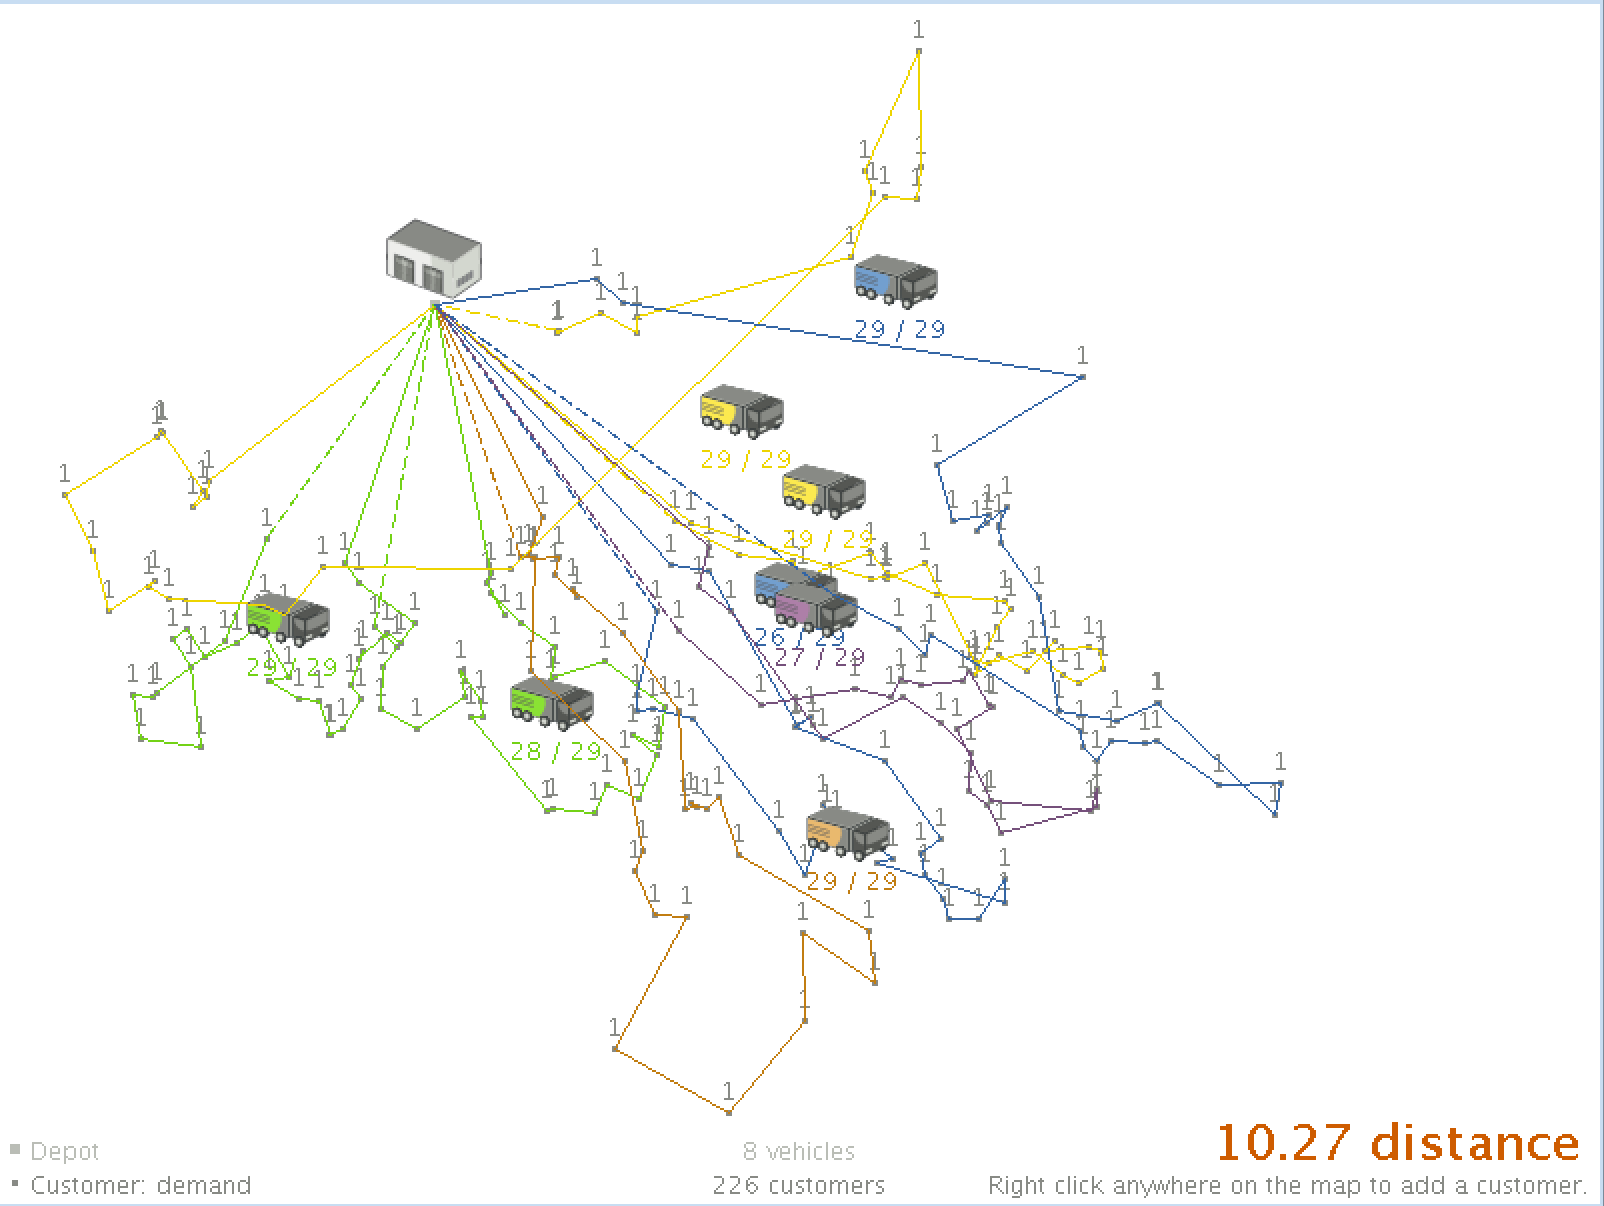
\includegraphics[width=1\textwidth]{227-cvrp.png}
    \caption{Visualisation of CVRP Model}
\end{figure}

\begin{figure}[!ht]
  \centering
    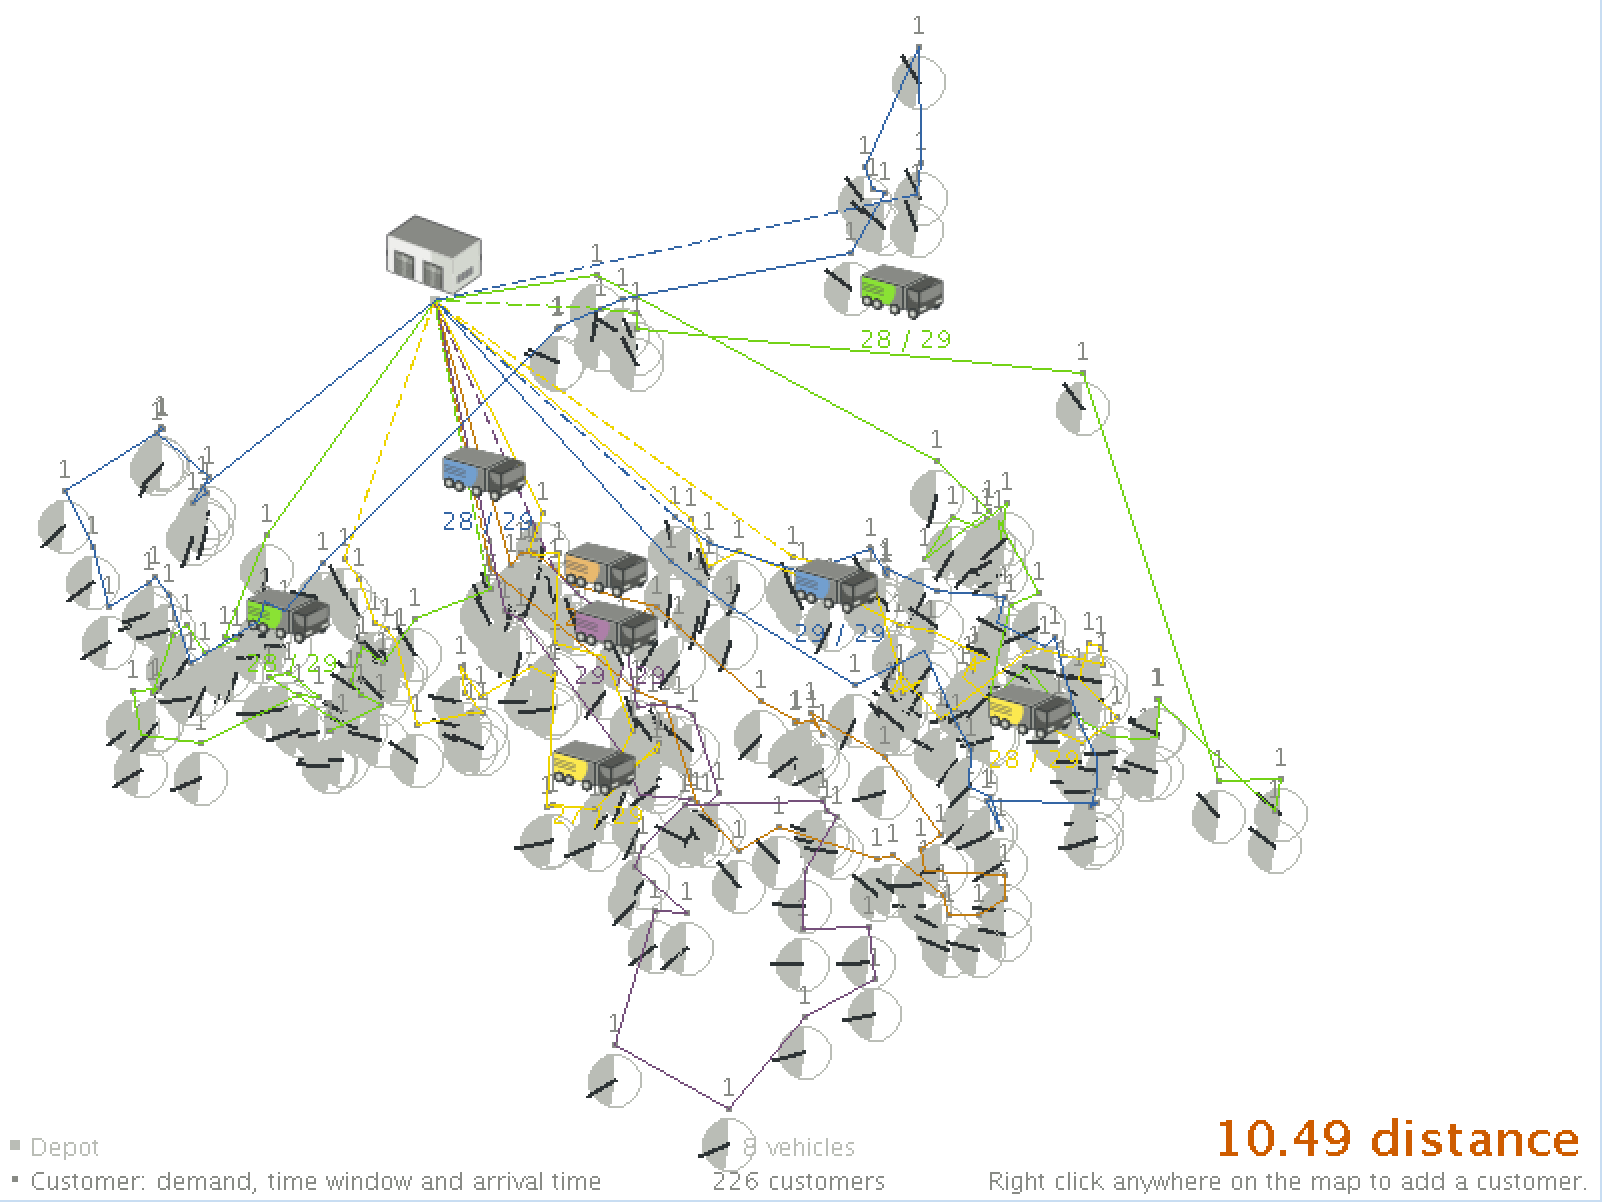
\includegraphics[width=1\textwidth]{227-cvrptw.png}
    \caption{Visualisation of CVRPTW Model}
\end{figure}

\section{Discussions}
\begin{enumerate}
\item Performance analysis of LP tools. Overall, Gurobi outperforms or-tools and optaplanner on all the models with
benchmark datasets. The optimal results obtained are even better than the known solution. We assume that the model is
correct, given the fact that it performs well on the test instance.
Or-tools underperforms on all cases using cheapest arc heuristics. Using different heuristics does not
improve the results and may take too long to terminate. Optaplanner gives a solution that is close to the best known result
 and gives the best performance for P-VRP-60, which indicates that it may be more suitable to use on a given problem.
 here are some pros and cons of using the tools, we only comment on the its application in VRP based problems.

\item Why Optaplanner? There are a few reasons to choose optaplanner. Firstly, it yields the best solution for the instance
of CVRP based on the given problem. It is easy to create a model and free: these two criteria is important, considering that
the requests made by the company.

\item talk about parameter estimation. We estimate the parameters such as the number of vehicles and its maximum capacity by trial
and error. There are 227 nodes, so the minimum number of edges to traverse all the edges once is 227. So, we get the combination of vehicles
and capacity by multiplying them such that the product is slightly greater than 227. In our analysis, using 8 vehicles and with 29 capacity
yields the best result.

\item How accurate is the model compared to the real life scenario?
 We are using air distance, which does not accurately present
the roads in traffic as they are never straight. This may undermine the quality of the solution
 In addition, we need to use the haversine function on the routes to get the distance covered in km. However, this solution
 would definitely be efficient enough to save the company money when utilised, as opposed to using manual route planning.

\item Advantages and Disadvantages of using each tool and suggest which tool to use given user profile.
\end{enumerate}

\begin{table}[!ht]
\centering
\caption{My caption}
\label{my-label}
\begin{tabular}{|l|p{0.2\textwidth}|p{0.2\textwidth}|p{0.3\textwidth}|}
\hline
Tools       & Advantages & Disadvantages & Comments \\ \hline
Gurobi      & High performance, good APIs to interface other languages, easy to install, and more control on model implementation.
            & Costs money when used for business and relatively hard to use
            & This tool is suitable for companies with sizeable budget on the data analysis department and more experienced OR analysts. \\ \hline
Or-tools    & good APIs to interface popular languages,free, open source  &  Relatively poor performance and hard to install  & This tool is suitable for hobbysts and experienced programmers who would like to look at examples and optimise their own solver\\ \hline
Optaplanner &  Good performance, comes with GUI, free, open source, easy to model formulation &     only support Java     & Good tool for learning how to solve planning problems. Can also be used at enterprise level...  \\ \hline
\end{tabular}
\end{table}

\section{Review}
Review this chapter... balh dih blah lorem ipsum dolor amet
